\documentclass{standalone}
\begin{document}
	\section{Time Performances}
	As I've said before the time performances are a relevant parameter of this pipeline. In this section I will discuss the segmentation time.  Since for this work I've to segment several scans (over than $100$), I've performed the  two main step (lung extraction and labeling) seprately, and compute the time segmentation time for each slice and phase. The timing for the training step was not measured since this step is performed only once, so doesn't affect the total segmentation time.\\
	The time performances are measured by performing the segmentation on the DIFA servers.\\
	
	In \figurename\,\ref{fig:Timing} I've plotted the segmentation time versus the number of slices.
	 
	\begin{figure}[h!]
		\centering
			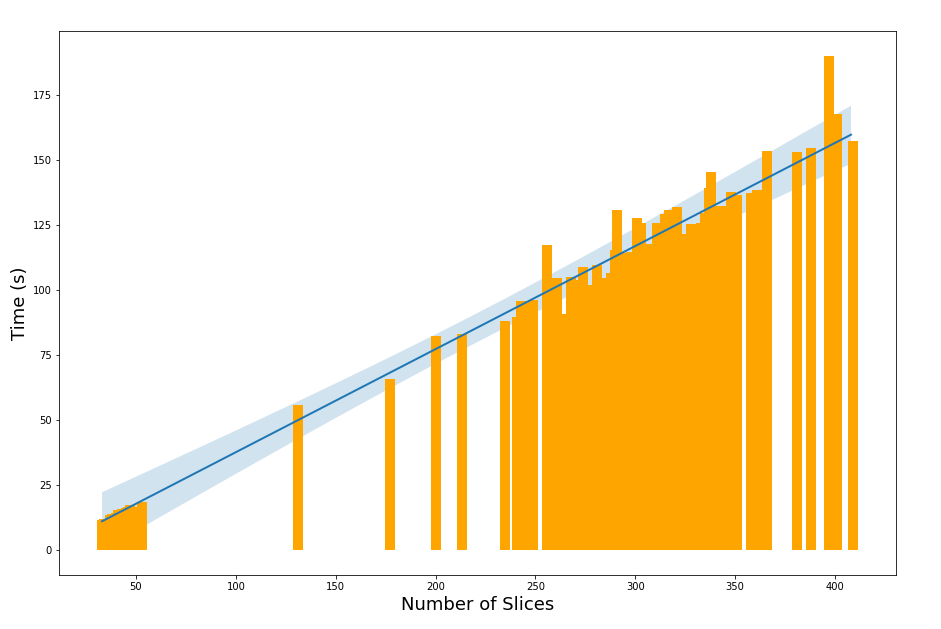
\includegraphics[scale=.75]{Timing.png}
			\label{fig:Timing}\caption{Total lung segmentation time vs number of slice for each scan of each dataset}
			
	\end{figure}
	As we can see the segmentation time increase linearly with the number of slices, so in order to measure the time for a single slice I've performed a linear fit and compute the angular coefficient. From this analysis I've measured that the segmentation time $0.40\,sec$ for each slice of the CT scan.\\
	
	After that I've measured the time for the labeling process, using the same procedure as before.
\end{document}

